%%%%%%%%%%%%%%%%%%%%%%%%%%% asme2ej.tex %%%%%%%%%%%%%%%%%%%%%%%%%%%%%%%

%%%%%%%%%%%%%%%%%%%%%%%%%%%%%%%%%%%%%%%%%%%%%%%%%%%%%%%%%%%%%%%%%%%%%%

%%% use twocolumn and 10pt options with the asme2ej format
\documentclass[twocolumn,10pt]{asme2ej}
%
\usepackage{epsfig} %% for loading postscript figures

%% The class has several options
%  onecolumn/twocolumn - format for one or two columns per page
%  10pt/11pt/12pt - use 10, 11, or 12 point font
%  oneside/twoside - format for oneside/twosided printing
%  final/draft - format for final/draft copy
%  cleanfoot - take out copyright info in footer leave page number
%  cleanhead - take out the conference banner on the title page
%  titlepage/notitlepage - put in titlepage or leave out titlepage
%
%% The default is oneside, onecolumn, 10pt, final


\title{MATH 371 Fall Quarter MCM 2019 Problem B}


\begin{document}

\maketitle


\begin{abstract}
{\it This is the abstract. This is the thing we're going to spend a LOT of time writing, it's very important. We still need to write the abstract and the introduction
}
\end{abstract}

%\begin{nomenclature}
%\entry{A}{You may include nomenclature here.}
%\entry{$\alpha$}{There are two arguments for each entry of the nomemclature environment, the symbol and the definition.}
%\end{nomenclature}

%The primary text heading is  boldface and flushed left with the left margin.  The spacing between the  text and the %heading is two line spaces.

\section{Introduction}
In the aftermath of natural disasters such as the Puerto Rico hurricane in 2017, many non-governmental organizations will be tasked with providing relief to strained health-care facilities and damaged infrastructure. The need for methods that can provide efficient and effective distribution of medical supplies and surveillance of the damaged area has been evident in many past natural disasters. In response to this growing need many companies, including HELP, Inc. have began investigating a method of supply dispersal and surveillance involving a fleet of unmanned drones. HELP Inc. has selected 8 candidates for a drones system designed to repond to natural disasters in Puerto Rico, called "DroneGo." There are also 3 specific medical packages designed for supplementing medical equipment for local hospitals in Puerto Rico and plans for storage locations for the required drones and medical packages. The drones also have a secondary task of surveying the damaged area for responders to know the terrain into which they are going. \\
The unique ability of aerial drones to survey difficult terrain without risk of harm could be found invaluable for responders. Drones can navigate through collapsed buildings and other infrastructure which would be impossible for any ground vehicle or any human (without extensive equiptment) to navigate. Additionally, aerial drones are a popular solution due to the fact that in many countries most effected by natural disasters, a large portion of the population does not live close enough to a road for a ground delivery system to be effective (need citation)\\
Much of the technology involving drone delivery has been advanced by the parcel delivery industry (need citation) and many of these systems has similar needs and considerations such as ability to land and drop cargo, cargo capability, and effective navigation in different environments (need citation). However, there are several considerations unique to the problem of medical supply delivery and reconnaissance; specifically careful handling of precious cargo, navigating damaged infrastructure, regular reusability, camera field of view and camera obstruction. Drones have been used for healthcare relief in the past, specifically in Haiti, the Dominican Republic, and New Guinea (need citation) but these have not been large scale, coordinated fleets. \\
The use of unmanned aerial drones for surveillance has been widely investigated and effectively used for military and civilian applications (need citation) with various types of drones being used depending on the requirements of the situation. This particular use of drone surveillance would most align with military use being more focused on quick detection of major terrain features and the presence of people. \\
Optimization of aerial drone path algorithms have also been investigated (need citation) with many different algorithms being found for road tracking (need citation) flight path efficiency (need citation) and navigating a changing environment. In navigating a changing environment, there becomes considerations of instrumentation on the drone and the drones ability to interpret those instruments. Similar algorithms have been widely used for developments in self-driving cars (need citation) where a dynamic path allocation and navigation is necessary. \\
The long term considerations of having a drone system that is constantly at the ready involve drone storage, drone power, changing environmental effects over long periods of time, and drone deployment. Many investigations have been done into various drone deployment methods (need citation) but for the DroneGo system, HELP Inc. has selected large storage containers to be kept on Puerto Rico soil in which the drones will be stored and from which the drones will deploy.

\section{Ideation}
We identified two significant problems to focus on in our model: packaging the drones and medi-packs to be deployed in the disaster area, and routing the drones to deliver necessary supplies according to the requirements from the delivery locations in attachment 4. We generalized a solution early on that involved algorithmically optimizing the packing space in each cargo container and modeling many routes to choose an ideal route based on a cost function, thereby eliminating two degrees of freedom. The remaining freedom is in choosing which drone type to use, which we determined could be implemented in the flight-path algorithm.

In this problem, there is already a lot of information established: the dimensions of all interacting products are fully defined, the performance capabilities of the drones are known, and the exact locations of delivery locations in the form of latitude and longitude points are provided. We used all this information to our advantage to narrow the scope of the problem and allow us more time to model the specific operational flow of our disaster response system. Despite this, however, several assumptions and simplifications were made in our model to reduce complexity which are outlined below.

\section{Assumptions}

\begin{itemize}
	\item Scheduling
	\begin{itemize}
		\item[--] Only the minimum supplies required daily are delivered to delivery locations, i.e. no rotating schedules and stockpiling of supplies to avoid needing to deliver to each daily
		\item[--] Additional time for operations is not considered: no time is needed to be spent in between flights for loading supplies or recharging the drones, and no time is needed to land and deliver supplies at delivery locations
	\end{itemize}
    \item Packing
    \begin{itemize}
    	\item[--] Elements can be stacked in any configuration without structural limitations
    \end{itemize}
	\item Flight path routing
	\begin{itemize}
		\item[--] Paths are perfectly straight
		\item[--] Every path only has either the delivery location or storage container as origin and destination
		\item[--] Paths are modeled in two dimensions i.e. no altitude changes are considered
		\item[--] Not considering effects of having multiple drones flying at once
	\end{itemize}
	\item Environmental effects
	\begin{itemize}
		\item[--] Influences from wind are neglected
		\item[--] The drones are assumed to be unobstructed by terrain
		\item[--] The drones do not experience any malfunctions
		\item[--] The earth’s curve is neglected
	\end{itemize}
\end{itemize}


\section{Overview of Algorithms}
 
 
\subsection{Flight Path Algorithm}
The flight path algorithm inputs the coordinates of each delivery location and its required medi-packs, information about each drone type, and assumes the starting location to be (0,0). It generates a list of all possible configurations of flight paths, each one represented as a vector of 2D lines. Any configurations that do not visit required hospitals , otherwise fail to meet delivery requirements, or cannot be sufficiently packed into the storage container(s) are eliminated from the list. A cost function that divides the total number of packages delivered by total distance over maximum speed is applied to the remaining list of configurations to find the least expensive flight paths. The algorithm is written in MATLAB and outputs a graph which represents the flight paths as lines and delivery locations as points, and the program outputs the total number of optimized flight paths found in the console.

The algorithm does not apply any calculation to determine how many medi-packs can fit in each drone configuration: analysis was done by hand to evaluate this for each drone type, and the maximum number of medi-packs that each drone can carry is hardcoded into the algorithm. 

Many limitations from this algorithm become immediately apparent: the real-life terrain that would be faced by the drones is ignored in favor of an ultra-simple “by the crow flies” model of flight. By utilizing this approach, the model also invalidates any capability of maximizing surveillance of roadways on the island of Puerto Rico, which was identified as a major focus for the DroneGo disaster response system.

\subsection{Packing Algorithm}
A packing algorithm is used to determine whether the materials necessitated by each flight configuration can be spatially packed into the dimensions of a standard ISO dry cargo container. The algorithm inputs the dimensions of each drone type and each medipack, and outputs a simple boolean expressing whether the configuration will fit or not. The algorithm  inputs the items into the cargo area by creating columns with base dimensions defined by the packages, and checks whether each new package can be stacked in an existing column before resorting to making a new column. Each package is only considered for one optimal orientation which is hardcoded prior. If the algorithm still has packages left to pack, but cannot create any more columns, it will return a 0.

\subsection{Cost Function}
Our cost function is described by the following formula, evaluating for a via flight plan and drone configuration.
\[
C = \alpha \frac{P}{\sum{t}} - \beta \frac{S}{100000}
\]
Where $P$ represents the total medpacks delivered, $\sum{t}$ is an estimate of the time for all the flights to occur, and $S$ represents the space left after packing all the drones (computed via the packing algorithm). Also, $C$ is our cost function output, the cost. The factor of $100000$ dividing $S$ is there to adjust the units of $S$ (it being on the order of $10^5$ while $\frac{P}{\sum{t}}$ is on the order of $10^0$) The time estimates are computed via the basic kinematic equation assuming constant speed, $\sum{t}=\sum{\frac{d}{v_d}}$ summed over all drone flights in the given plan. Here $d$ is distance traveled in a specified flight and $v_d$ is the max speed of the drone flying. This estimate of the time taken for a flight is assuming the drone is flying at max speed the whole way, and assuming equality of the time taken to fly to the hospital, and the time to fly back. The assumption of perfectly sequential ordering of the flights allows us to sum the times of individual flights to get the total time.

\section{Results and Analysis}

\subsection{Model output}
The typical model output expected to be used by the customer specifies several drone movements and a drone configuration. Each movement is a possible opportunity for a single drone to make one flight. A configuration specifies how many drones and of what types the drone are. In our simplified drone path algorithm, each movement is a straight line path from the starting location to the hospital specified, performed by a specified drone. Our final output is thus a single series of movements and a single configuration, corresponding to the most optimized plan, as determined by our cost function. In figure XXX, an example of an optimized model output is shown (need to include parameters it ran with in the figure description). \\
Although it is not depicted in the figure, a model run will product viable flight plans such as the one below, each with its own cost value. In the course of using our model, it may become necessary to select a sub-optimal flight plan due to limiting factors not taken into account with our model. Therefore it is necessary to statistically analyze all the cost function outputs for a given model run near the minimum (representing the most optimal flight plan). This analysis was done for studies of parameter sensitivity as well as for directly comparing model outputs.

% TODO: \usepackage{graphicx} required
\begin{figure*}
	\centering
	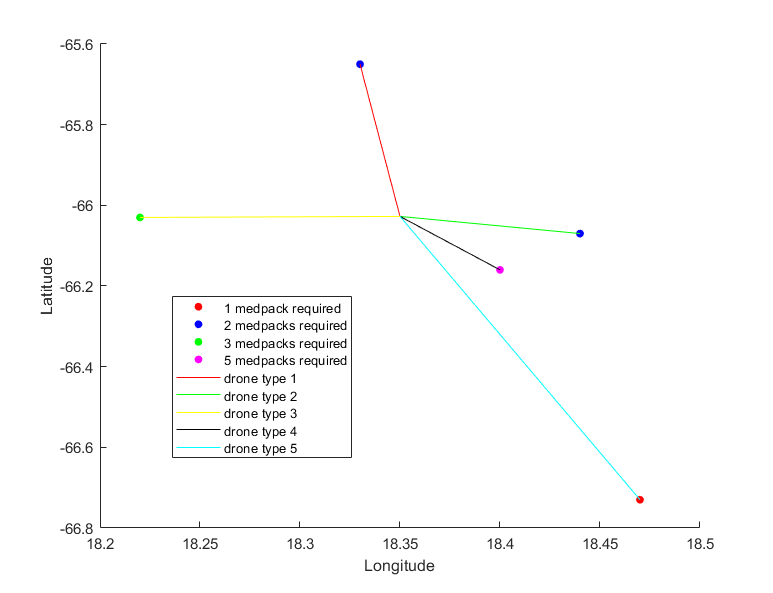
\includegraphics[width=0.7\linewidth]{../example_flight_plan}
	\caption[Fig 1.]{Example optimized flight plan, ran with drone fleet size of 5, starting location 1, 5 allowed movements, and $\gamma$ = 2}
	\label{Fig 1.}
\end{figure*}

\subsection{Parameter sensitivity}
The model output, specifically the outputs of the cost function were analyzed after varying different parameters to find reasonable values for further analysis. The metric used for comparing the effectiveness of our model outputs is a measure of how many viable flight paths are produced with a cost function value near the minimum. The parameters we varied were the different valid storage bin configurations, the number of allowed movements in a flight plan and the number of drones in a fleet. \\
As the output of our storage location sub-model, we had 15 possible configurations for storage bin locations (which we limited to 2 storage bins). This limit was imposed as to be the minimum number of storage bins needed to understand the effects of having multiple storage bins and the effect that changing those configurations would have on the model output. The results of this study are shown in figure XXX. \\
---analysis of that figure and what it means for model sensitivity of storage location --- \\
The number of allowed movements in the flight plan was limited by our hospital requirements. For example, the sum of all required medipacks for a day was 13, so no configuration of only drone B (which can hold only 1 medipack) can have less than 13 movements. Thus, because our max drone capacity was 2 medipacks, our minimum number of allowed movements in a flight plan was 7. Our model mostly did not consider the interaction between the number of allowed movements and the number of drones in the fleet due to our assumption that every drone can make as many or as little trips as possible in a day. However, there may be an additional interaction between these quantities in terms of the optimized flight plan but our parameter sensitivity was limited to studying sensitivity of individual parameters and not their interactions. \\
Due to fundamental limitations of our models implementation we cannot investigate the outputs of infinitely many allowed movements. But this is a realistic view of the problem because in a single day, you cannot have infinitely many drone movements without infinitely many drones. Our selected parameter range and outputs are shown in figure XXX. \\\
---analysis of the figure and what it means for model sensitivity of allowed movements ---


\subsection{Limitations/ Further work}
The cost function developed is limited in that if favors solution with fewer drones even when the combined effort of those many drones may be more effective than the combined effort of fewer drones. This arises from our assumption of sequential drone paths. A fleet of many drones may be monetarily expensive but could lead to extremely efficient in delivering medipacks due to all the drones delivering at once. This limitation would be further amplified in larger-scale drone fleet models, and for that use, an more complex metric for medipack delivery efficiency is recommended. \\
Furthermore, our cost function did not take into account mapping of disaster terrain. This can be reconciled by adjusting our optimized model output after it has been optimized to the current cost function. It can then be adjusted to add curvature, surveying different areas of land according to a certain metric, representing how far it may deviate from the most simple path (a straight line). The main limitation of performing this adjustment after the main optimization is that adding this curvature will increase $\sum{t}$ as defined in the cost function and may increase $sum{t}$ unevenly across different viable flight paths. This could lead to a different optimized flight plan after the curvature would have been added. Thus, by adding the curvature after optimized by our cost function we lose the guarantee that our output is the most optimized under our cost function. \\
Our assumption of perfectly flat 2D terrain without any need to alter the drone path due to obstructions causes us to lose the fundamental aspect of navigation in our drones. Due to the nature of natural disasters, it would be impossible to predict the conditions in which the drones must navigate through after a natural disaster and therefore a stochastic method of modeling terrain obstructions and required alternate routes. This would also be an effective measure of the DroneGo system's ability to operate in any condition that comes up. Whether the implementation of a stochastic terrain model would on average alter the optimized outputs of the model would be an interesting investigation. \\




\end{document}
